%% -*- ispell-local-dictionary: "es" -*-

\documentclass[a4paper,twoside]{article}
\usepackage[utf8]{inputenc}
\usepackage[spanish]{babel}
\usepackage{indentfirst}
\usepackage{fancybox}
\usepackage{epsfig}
\usepackage{tabularx}
\usepackage{sectsty}
\usepackage{amsmath}
\usepackage{float}
\usepackage{listings}
\usepackage{color}
\usepackage{subfigure}
\usepackage[colorlinks=true,linkcolor=blue,urlcolor=blue]{hyperref}
\usepackage{placeins}
\usepackage{verbatim}
\usepackage[table]{xcolor}
\usepackage{multirow}
\usepackage{rotating}
\usepackage{pdflscape}
%\usepackage{natbib}


\newcolumntype{R}{>{\raggedleft\arraybackslash}X}
\newcolumntype{C}{>{\centering\arraybackslash}X}


\marginparwidth 0pt     \marginparsep 0pt
\topmargin   0pt        \textwidth   6.5in
\textheight 23cm
% Margen izq del txt en impares.
\setlength{\oddsidemargin}{.0001\textwidth}
% Margen izq del txt en pares.
\setlength{\evensidemargin}{-.04\textwidth}
% Anchura del texto
\setlength{\textwidth}{.99\textwidth}


\lstset{ %
  language=Java,                     % choose the language of the code
  basicstyle=\scriptsize\ttfamily,               % the size of the fonts that are used for the code
  numbers=left,                   % where to put the line-numbers
  numberstyle=\tiny,              % the size of the fonts that are used for the line-numbers
  stepnumber=5,                   % the step between two line-numbers. If it's 1 each line will be numbered
  numbersep=5pt,                  % how far the line-numbers are from the code
  backgroundcolor=\color{white},  % choose the background color. You must add \usepackage{color}
  showspaces=false,               % show spaces adding particular underscores
  showstringspaces=false,         % underline spaces within strings
  showtabs=false,                 % show tabs within strings adding particular underscores
  frame=single,	                  % adds a frame around the code
  tabsize=2,	                  % sets default tabsize to 2 spaces
  captionpos=t,                   % sets the caption-position to bottom
  breaklines=true,                % sets automatic line breaking
  breakatwhitespace=true,         % sets if automatic breaks should only happen at whitespace
  escapeinside={\%*}{*)},         % if you want to add a comment within your code
}


\def\assignedcell{\cellcolor[gray]{0.9}}
\def\rangecell{\cellcolor[gray]{0.7}}
\def\filtercell{\cellcolor[gray]{0.5}}
\def\nocell{\cellcolor[gray]{0.3}}



\author{Barros Barros, Ismael \\
  Fernández Núñez, Daniel \\
  Iglesias Fraga, David}
\date{\today}



\title{Práctica Java POJO -- Sitio web de apuestas deportivas \\ Integración de Sistemas 2009-2010}
\pagenumbering{arabic} \pagestyle{myheadings} \markboth{Integración de Sistemas 2009-2010}{Práctica Java POJO}

\begin{document}
\maketitle
\cleardoublepage
\tableofcontents
\cleardoublepage

\section{Arquitectura global}


\begin{figure}[H]
  \centering
  \caption{Diagrama de arquitectura}
  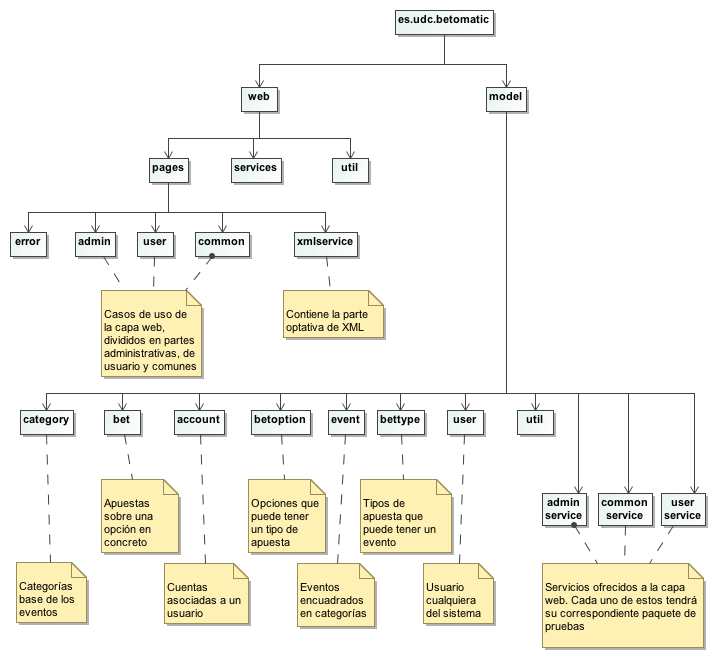
\includegraphics[width=\textwidth]{../uml/Diagramas_it2_imgs/Free_Form_Diagram__Arquitectura.png}
\end{figure}


\newpage
\section{Modelo}


\subsection{Clases persistentes}

\begin{figure}[H]
  \centering
  \caption{Diagrama de clases persistentes}
  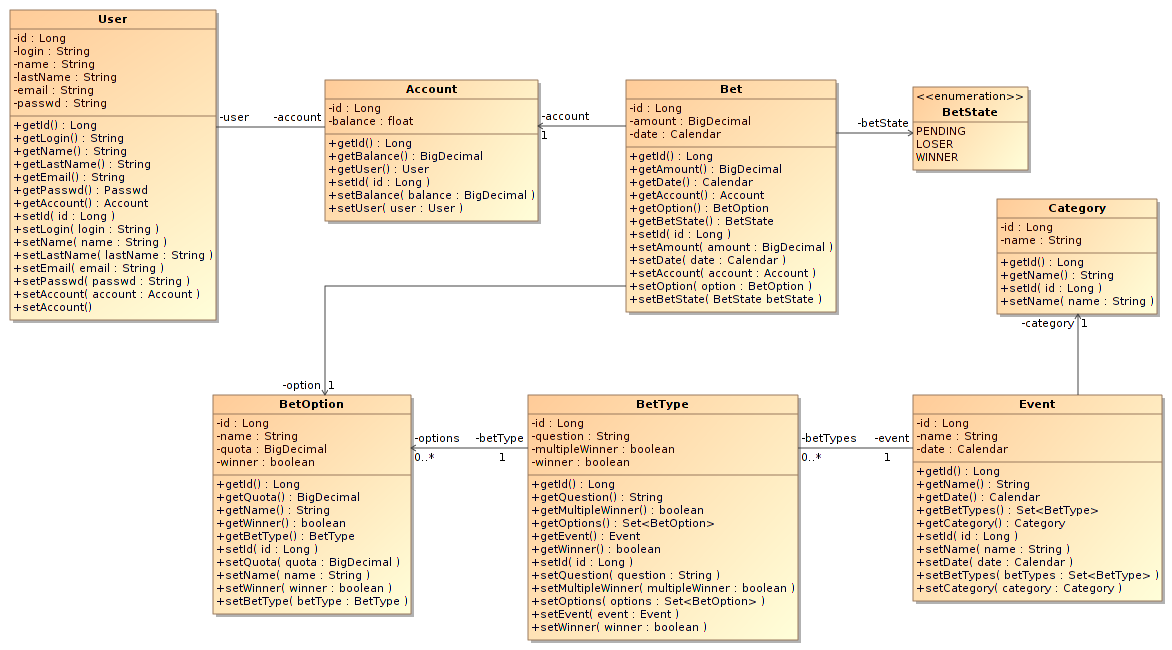
\includegraphics[width=.85\textheight,angle=90]{../uml/Class_Diagram__Clases_persistentes.png}
\end{figure}

\newpage
\subsection{Interfaces de los servicios ofrecidos por el modelo}

\begin{figure}[H]
  \centering
  \caption{Interfaces de los servicios}
  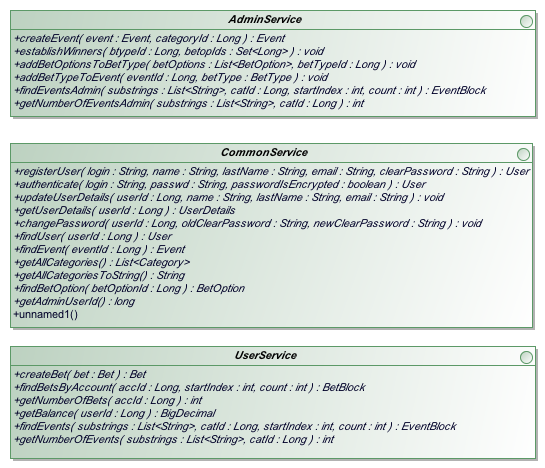
\includegraphics[scale=.7]{../uml/Diagramas_it2_imgs/Class_Diagram__Interfaces.png}
\end{figure}

Se ha clasificado la funcionalidad del sistema en tres servicios:

\begin{description}
\item[Servicio de administración:] Contiene la funcionalidad específica requerida para la administración del sistema.
\item[Servicio de usuario:] Contiene la funcionalidad referida a los clientes del sistema.
\item[Servicio común:] Contiene la funcionalidad que no pertenece necesariamente ni al administrador ni al cliente.
\end{description}



\newpage
\subsection{Diseño de un DAO}

\begin{figure}[H]
  \centering
  \caption{Diagrama de clases del DAO de la clase User}
  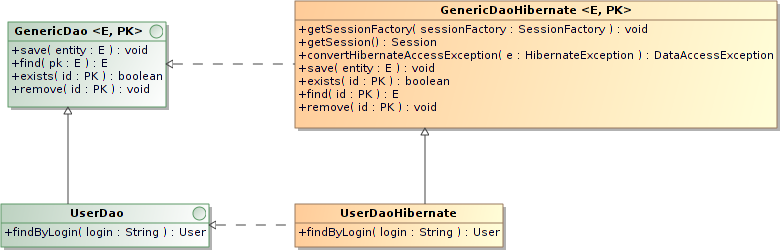
\includegraphics[width=\textwidth]{../uml/Class_Diagram__Clases_UserDao.png}
\end{figure}


%\newpage
\subsection{Diseño de un servicio del modelo}

%% \begin{figure}[H]
%%   \centering
%%   \caption{Diagrama de clases del servicio UserService}
%%   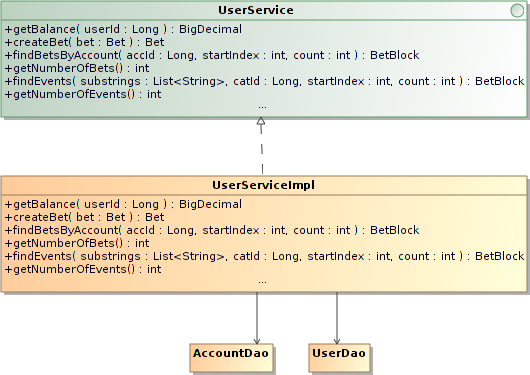
\includegraphics[width=\textwidth]{../uml/Class_Diagram__Clases_UserService.png}
%% \end{figure}

\begin{figure}[H]
  \centering
  \caption{Diagrama de clases del servicio UserService}
  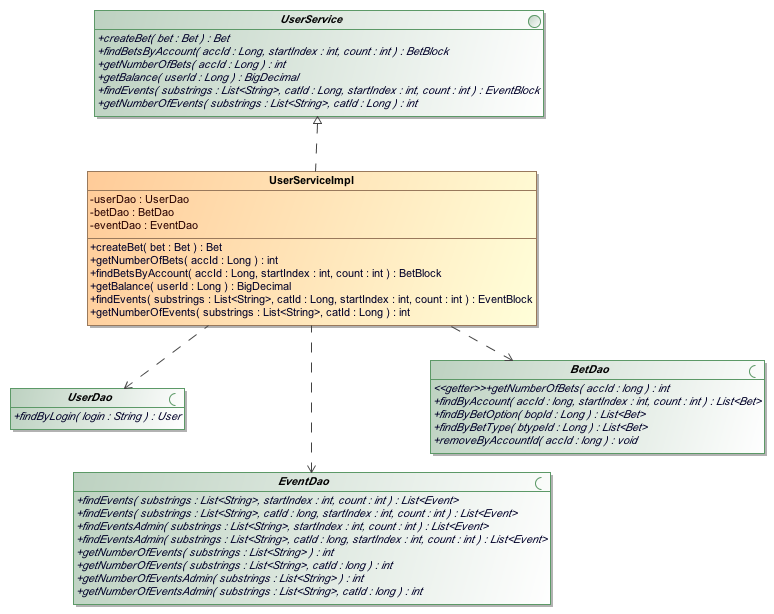
\includegraphics[width=\textwidth]{../uml/Diagramas_it2_imgs/Class_Diagram__Servicio.png}
\end{figure}

\begin{figure}[htbp]
  \centering
  \caption{Diagrama de secuencia para el registro de usuario en el modelo}
  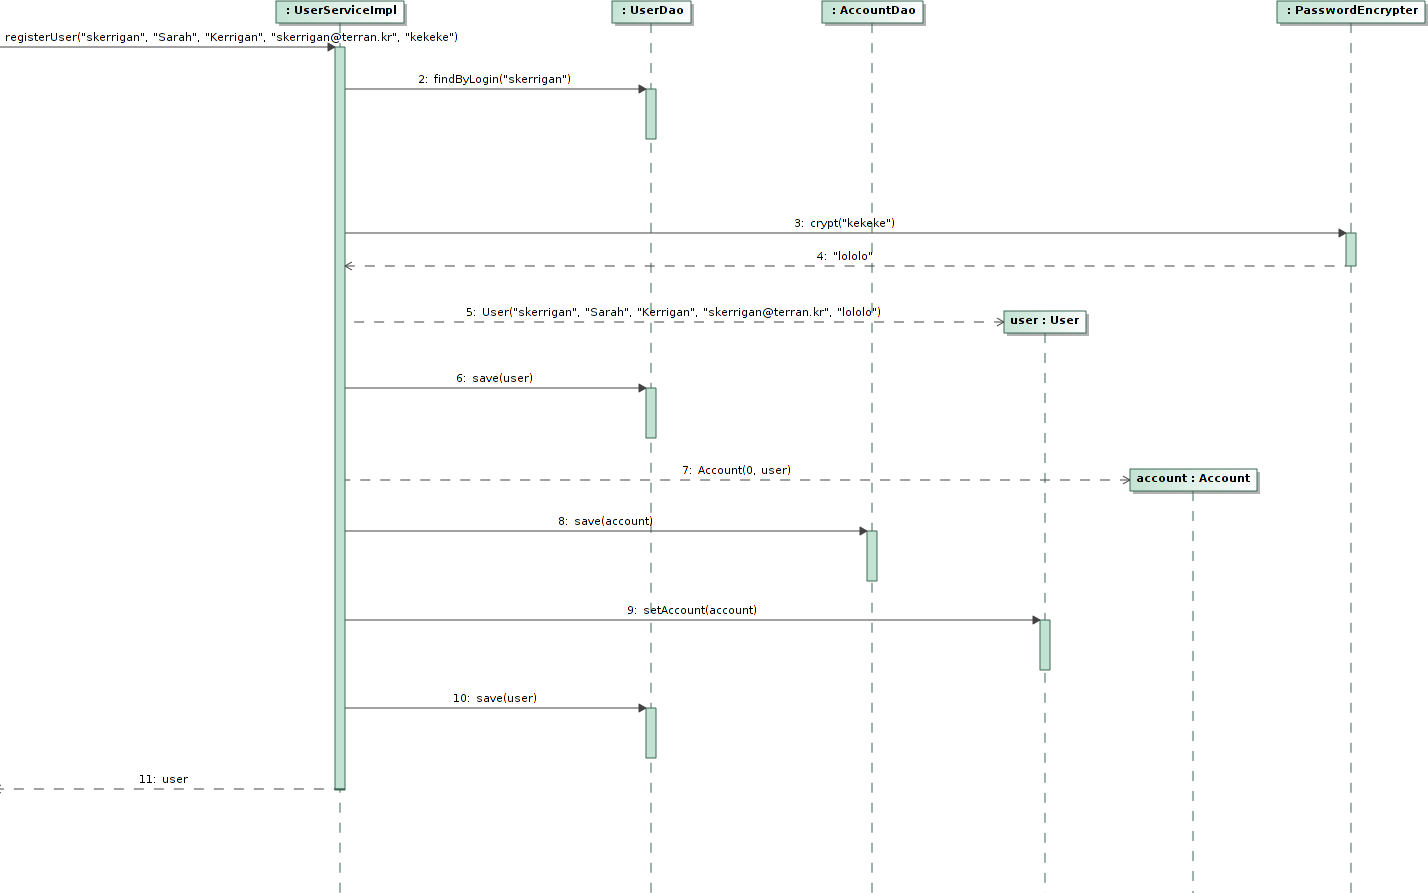
\includegraphics[width=\textheight,angle=90]{../uml/Sequence_Diagram__Secuencia_UserService__Secuencia_UserService.png}
\end{figure}



%\subsection{Otros aspectos}


\newpage
\section{Interfaz gráfica}

\begin{figure}[H]
  \centering
  \caption{Diagrama de secuencia del registro de un usuario en la interfaz gráfica}
  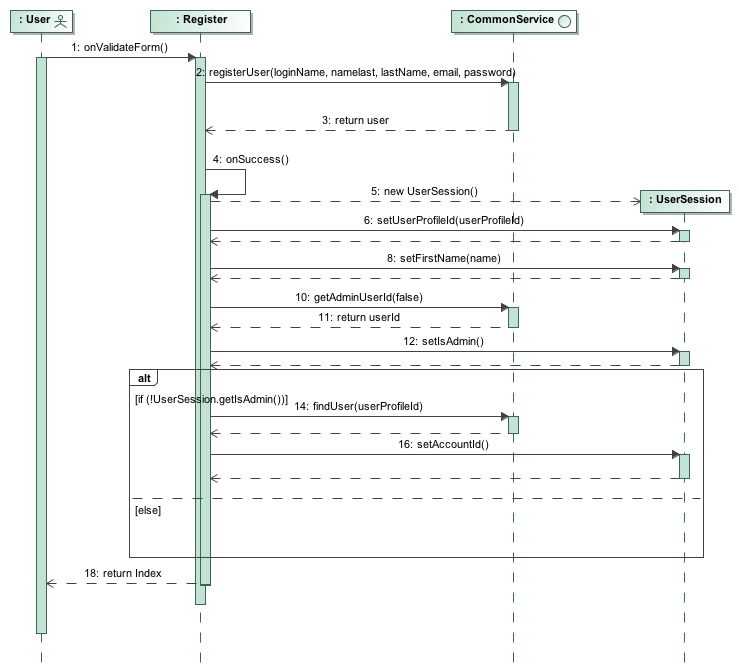
\includegraphics[width=\textwidth]{../uml/Diagramas_it2_imgs/Sequence_Diagram__SecuenciaWeb_registro__SecuenciaWeb_registro.png}
\end{figure}


\newpage
\section{Servicios XML}

Se han implementado dos funcionalidades básicas en la interfaz XML del sistema:

\begin{description}
\item[Búsqueda de eventos.] Permite buscar eventos en base a una lista de palabras clave.
  
  El formato de la petición es:

\begin{verbatim}
  http://<servidor>/xmlservice/FindEvents[?keywords=<lista de palabras clave>]
\end{verbatim}

En caso de que la petición se procese adecuadamente, la respuesta será de la forma:

\begin{verbatim}
  <rsp stat="ok">
    <events>

      <event>
        <id>[identificador del evento]</id>
        <name>[nombre del evento]</name>
        <date>[fecha del evento]</date>
        <category>[categoría del evento]</category>
      </event>

      ...

    </events>
  </rsp>
\end{verbatim}

En caso de que ocurra un error procesando la petición, la respuesta será de la forma:

\begin{verbatim}
  <rsp stat="fail">
    <err msg="[mensaje de error]" />
  </rsp>  
\end{verbatim}




\item[Búsqueda de tipos de apuesta de un evento.] Permite obtener la lista de tipos de apuesta de un evento.
  
  El formato de la petición es:

\begin{verbatim}
  http://<servidor>/xmlservice/ShowBetTypes?eventId=<identificador del evento>
\end{verbatim}

En caso de que la petición se procese adecuadamente, la respuesta será de la forma:

\begin{verbatim}
  <rsp stat="ok">
    <betTypes>

      <betType>
        <question>[pregunta del tipo de apuesta]</question>
          <multipleWinner>[si el tipo de apuesta admite más de un ganador]</multipleWinner>
          <betOptions>

            <betOption>
              <name>[nombre de la opción]</name>
              <quota>[quota de la opción]</quota>
            </betOption>

            ...

          </betOptions>
      </betType>

      ...

    </betTypes>
  </rsp>
\end{verbatim}

En caso de que ocurra un error procesando la petición, la respuesta será de la forma:

\begin{verbatim}
  <rsp stat="fail">
    <err msg="[mensaje de error]" />
  </rsp>
\end{verbatim}


\end{description}



\section{Un apartado para las partes adicionales}

\begin{description}
\item[Pruebas de integración exhaustivas.]
  Debido a la alta variedad de posibles búsquedas y de casos de funcionamiento, se han realizado pruebas de integración exhaustivas sobre el caso de uso de búsqueda de eventos por parte de un usuario. Se han probado los siguientes casos:
  \begin{itemize}
  \item Búsquedas con palabras clave y sin categoría
  \item Búsquedas con palabras clave y con categoría
  \item Búsquedas sin resultados
  \item Búsquedas con palabras clave desordenadas
  \item Búsquedas con partes de palabras
  \item Búsquedas sin palabras clave o con la palabra clave vacía
  \item Búsquedas sin palabras clave pero con categoría
  \item Búsquedas que devuelvan varias páginas de resultados
  \item Comprobación de que no se muestran eventos que ya han comenzado
  \item Comprobación de que se ordenan correctamente los eventos por fecha
  \end{itemize}

\item[AJAX.]
  Se ha intentado dotar de una funcionalidad cercana a la de las aplicaciones de escritorio al caso de uso de realizar una apuesta. Para ello, se ha hecho uso del soporte de Tapestry para AJAX.

  La implementación involucra dos {\tt zones} y un {\tt block}. La primera {\tt zone} alberga la lista paginada de apuestas que el usuario ha realizado hasta la fecha. La segunda {\tt zone} está inicialmente vacía, y se rellenará con el formulario de apuesta contenido dentro del {\tt block} cuando el usuario hace click en una opción de apuesta.

  Los links se han dispuesto de tal modo que en lugar de recargar toda la página, recargan únicamente la zona correspondiente. Por ejemplo, los links de siguiente y anterior recargarán sólo la lista de apuestas, y los links de apostar recargarán sólo el formulario de apuesta.

\end{description}



\section{Compilación e instalación de la aplicación}

En un entorno con el software necesario instalado y configurado correctamente se han de seguir los siguiente pasos para compilar e instalar la aplicación:

\begin{enumerate}
\item Situarnos en el directoria base del proyecto, donde se encuentra el fichero {\tt pom.xml}, y ejecutar ``{\tt mvn sql:execute package}''.
\item Copiar el fichero {\tt betomatic-X.X.X.war} a la carpeta {\tt apache-tomcat-6.0.20/webapps}.
\item Ejecutar el SGBD MySql mediante el siguiente comando: ``{\tt mysqld --defaults-file=\$HOME/.my.cnf}''
\item Ejecutar el Servidor Web Apache Tomcat mediante el siguiente script: ``{\tt apache-tomcat-6.0.20/bin/startup.sh}''
\item Se recomienda cambiar la contraseña de administrador, por defecto es ``admin''. Esto se puede realizar desde la interfaz web de la aplicación.
\item Para detener el Servidor Web, ejecute el siguiente script: ``{\tt apache-tomcat-6.0.20/bin/shutdown.sh}''
\item Para detener el SGDB MySql, ejecute: ``{\tt mysqladmin -u root shutdown}''
\end{enumerate}


\section{Problemas conocidos}

\begin{itemize}
\item Al realizar un usuario una apuesta, si introduce en el campo para la cantidad a apostar un número con formato erróneo, la aplicación ignora la solicitud sin dar un mensaje de error.
\item Cuando un usuario con balance insuficiente intenta realizar una apuesta, la aplicación ignora la solicitud sin dar un mensaje de error.
%\item checkboxes? al añadir betOption no comprueba quota hasta que se manda crear (y no al darle a new betoption)?? (no creo q sea necesario ponerlo)
\end{itemize}


\end{document}
